\chapter{Empirical study and results}
\label{cpt:result}
\section{Stock market description}
There are totally 261 trading days in 2016 of US stock market, this thesis selects 1,418 stocks of listing US companies that were traded in all trading days in 2016. Table~\ref{tab:industrytable} lists the titles of 55 industrial sectors corresponding to the summary level of BEA industry codes as well as the number of stocks in each of them.
\begin{longtable}{c|c} 
	\centering
	\textbf{Industrial Sector Title} & \textbf{Stock Count}  \\ \hline
	Banks, credit intermediation, and related activities & 214 \\ 
	Computer and electronic products & 173 \\
	Funds, trusts, and other financial vehicles	& 132\\
	Insurance carriers and related activities & 85 \\
	Chemical products & 76 \\
	Utilities & 64 \\
	Food and beverage and tobacco products	& 56 \\
	Fabricated metal products & 52 \\
	Securities, commodity contracts, and investments & 42 \\
	Broadcasting and telecommunications	& 42 \\
	Other retail & 38 \\
	Machinery&	36 \\
	Wholesale trade & 33 \\
	Motor vehicles, bodies and trailers, and parts & 32 \\
	Construction & 30 \\
	Computer systems design and related services & 27 \\
	Performing arts, spectator sports, museums, and related activities & 27 \\
	Miscellaneous professional, scientific, and technical services & 23 \\
	Petroleum and coal products & 16 \\
	Paper products & 15 \\
	Air transportation & 14 \\
	Data processing, internet publishing, and other information services & 14 \\
	Ambulatory health care services & 12 \\
	Plastics and rubber products & 12 \\
	Accommodation & 12 \\
	Administrative and support services & 11 \\
	Truck transportation & 11 \\
	Rental and leasing services and lessors of intangible assets & 10 \\
	Other transportation and support activities & 9 \\
	Publishing industries, except internet (includes software) & 8 \\
	Other transportation equipment & 8 \\
	Support activities for mining & 7 \\
	Other real estate & 7 \\
	Miscellaneous manufacturing & 7 \\
	Oil and gas extraction	& 6 \\
	Furniture and related products & 6 \\
	Electrical equipment, appliances, and components & 6 \\
	Rail transportation & 5 \\
	Textile mills and textile product mills & 5 \\
	Nonmetallic mineral products & 5 \\
	Transit and ground passenger transportation & 4 \\
	Waste management and remediation services & 3 \\
	Hospitals & 3 \\
	Wood products & 3 \\
	Printing and related support activities & 2 \\
	Motion picture and sound recording industries & 2 \\
	Nursing and residential care facilities & 2 \\
	Pipeline transportation & 2 \\
	Primary metals & 2 \\
	Apparel and leather and allied products & 2 \\
	Other services, except government & 1 \\
	Water transportation & 1 \\
	Legal services & 1 \\
	Social assistance & 1 \\
	Mining, except oil and gas & 1 \\
	\textbf{Total} & \textbf{1,418} \\
	\caption{Part of counts for US stocks by industry \cite{secwebsite}}
	\label{tab:industrytable}
\end{longtable}

It is not hard to see the composition of stock market are mainly dominated by the finance-related industry ("Banks, credit intermediation, and related activities", "Funds, trusts, and other financial vehicles", "Insurance carriers and related activities", "Securities, commodity contracts, and investments", etc.) and computer-related industry ("Computer and electronic products", "Computer systems design and related services", "Data processing, internet publishing, and other information services", "Electrical equipment, appliances, and components", etc.). The total numbers of finance-related industry and computer-related industry are over 473 and 220 respectively, which jointly take almost half of the number of total stocks. Therefore, it is necessary to use the formalised formula~ which divides the value by the number of stocks in its belonging industrial sector, punishing the connection from or to a node by the industry size, i.e., if a stock is in a large industry, it will need higher transaction flows to connect to other nodes in the network.

\section{Networks construction}
This thesis first generated matrices of normalised direct demand \textbf{A}, normalised direct requirement \textbf{B}, correlation coefficient \textbf{C} using formula~\ref{equ:eio_i}, \ref{equ:eio_o}, and \ref{equ:corr}.

Figure~\ref{fig:eio_transaction_density} from normalised direct demand \textbf{A} and normalised direct requirement \textbf{B} illustrates that the transaction densities decrease as threshold of normalised direct requirement and normalised direct demand increase, and their patterns are very similar with the same inflection point at around $threshold=0.136$ where the densities begin to decline. Therefore, the values of thresholds for normalised direct requirement and normalised direct demand are set to be equal, i.e., $\theta_{EIO}=\theta_{DD}=\theta_{DR}$, to filter the directed edges among the stock network.

\begin{figure}
	\begin{center}
		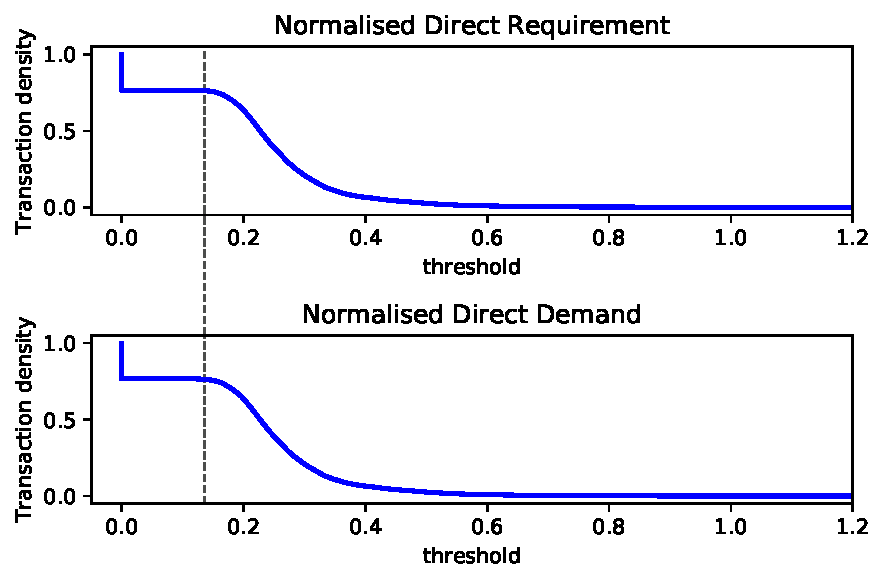
\includegraphics[width=14cm]{eio_transaction_density}
	\end{center}
	\caption{Transaction densities in EIO. The density of transactions drops vertically at the threshold of 0, which means nearly a quarter of values in the normalised direct demand matrix \textbf{A} and normalised direct requirement \textbf{B} are $0$. Then the two densities both decrease from the point around 0.136, and overall they follow a same pattern.}
	\label{fig:eio_transaction_density}
\end{figure}

Figure~\ref{fig:correlation_distribution} shows the distribution of stock price correlation coefficients has a shape complies to the normal distribution. Most correlation coefficients are vary from $-0.2$ to $0.85$ with the mean of $0.265$. Figure~\ref{fig:correlation_edge_density} also shows that the edge density drops dramatically as the correlation coefficient increases from $0$ to $0.50$. It implies that the prices of most stocks traded in NYSE and NASDAQ often fluctuate to the same direction, but the patterns are less similar to each other.

\begin{figure}
	\begin{center}
		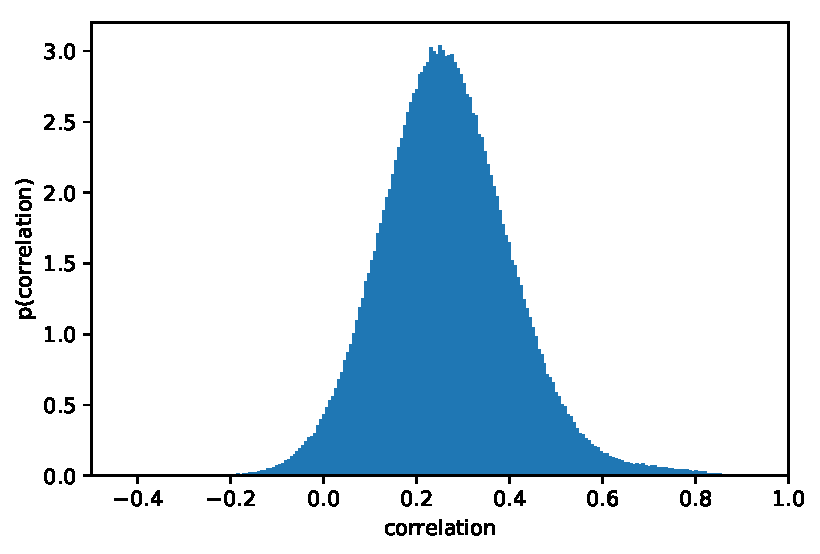
\includegraphics[width=14cm]{correlation_distribution}
	\end{center}
	\caption{Correlation coefficient distribution of stock price return. The minimum and maximum are $-0.687$ and $0.977$ and the mean is $0.265$. The distribution follows normal distribution.}
	\label{fig:correlation_distribution}  
\end{figure}

\begin{figure}
	\begin{center}
		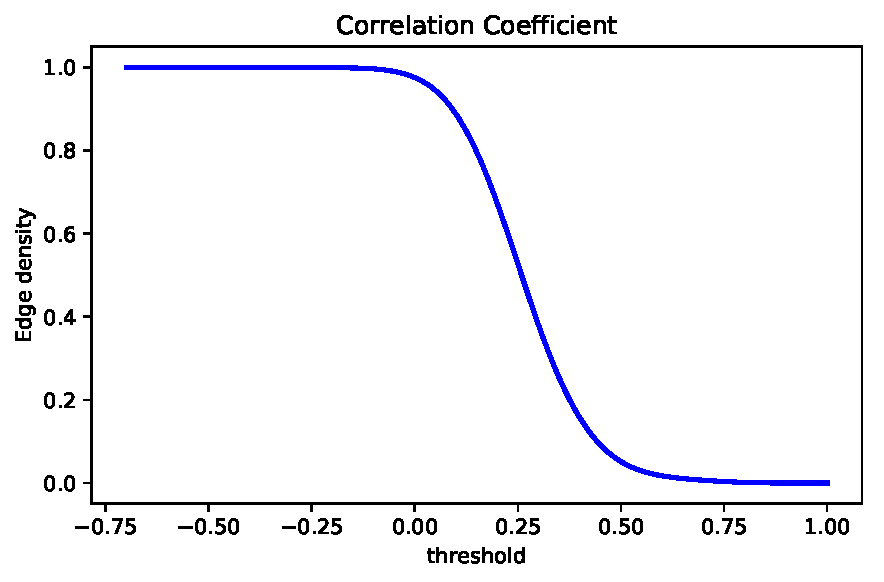
\includegraphics[width=14cm]{correlation_edge_density}
	\end{center}
	\caption[Edge density with correlation coefficient]{Edge density with correlation coefficient. The edge density drops dramatically as the correlation coefficient increases from $0$ to $0.50$.}
	\label{fig:correlation_edge_density}  
\end{figure}

Figure~\ref{fig:amounts_of_edges_threshold} shows the number of directed edges remain at the conditions of different value combinations of $\{\theta_{EIO}$, $\theta_{corr}\}$. When both of the thresholds set to be minimal at their own value range, i.e., $\theta_{EIO}=0$ and $\theta_{corr}=-1$, the number of directed edges is $N\times(N-1)=2,009,306$, while $N$ indicates the total number of nodes, which is $1418$. According to the figure~\ref{fig:amounts_of_edges_threshold}, the number of edges will be less than $100,000$, in which case the network has a density of lower than $5\%$, if $\theta_{EIO}\geq0.3545$ or $\theta_{corr}\geq0.5020$. 

\begin{figure}
	\begin{center}
		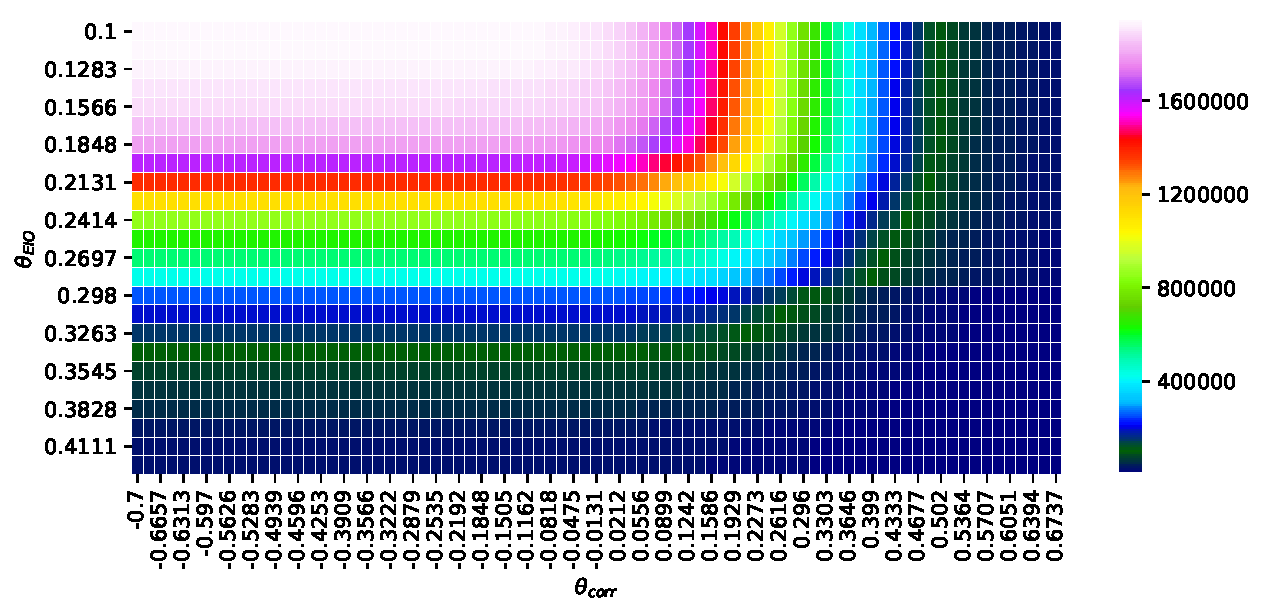
\includegraphics[width=15cm]{amounts_of_edges_threshold}
	\end{center}
	\caption{Heatmap of the numbers of directed edges per EIO-threshold and correlation-coefficient-threshold. The number of directed edges changes from the maximum to $0$ as $\theta_{EIO}$ decreases from $0.10$ to $0.45$ and $\theta_{corr}$ increases from $-0.70$ to $0.68$.}
	\label{fig:amounts_of_edges_threshold}  
\end{figure}

\begin{figure}
	\begin{center}
		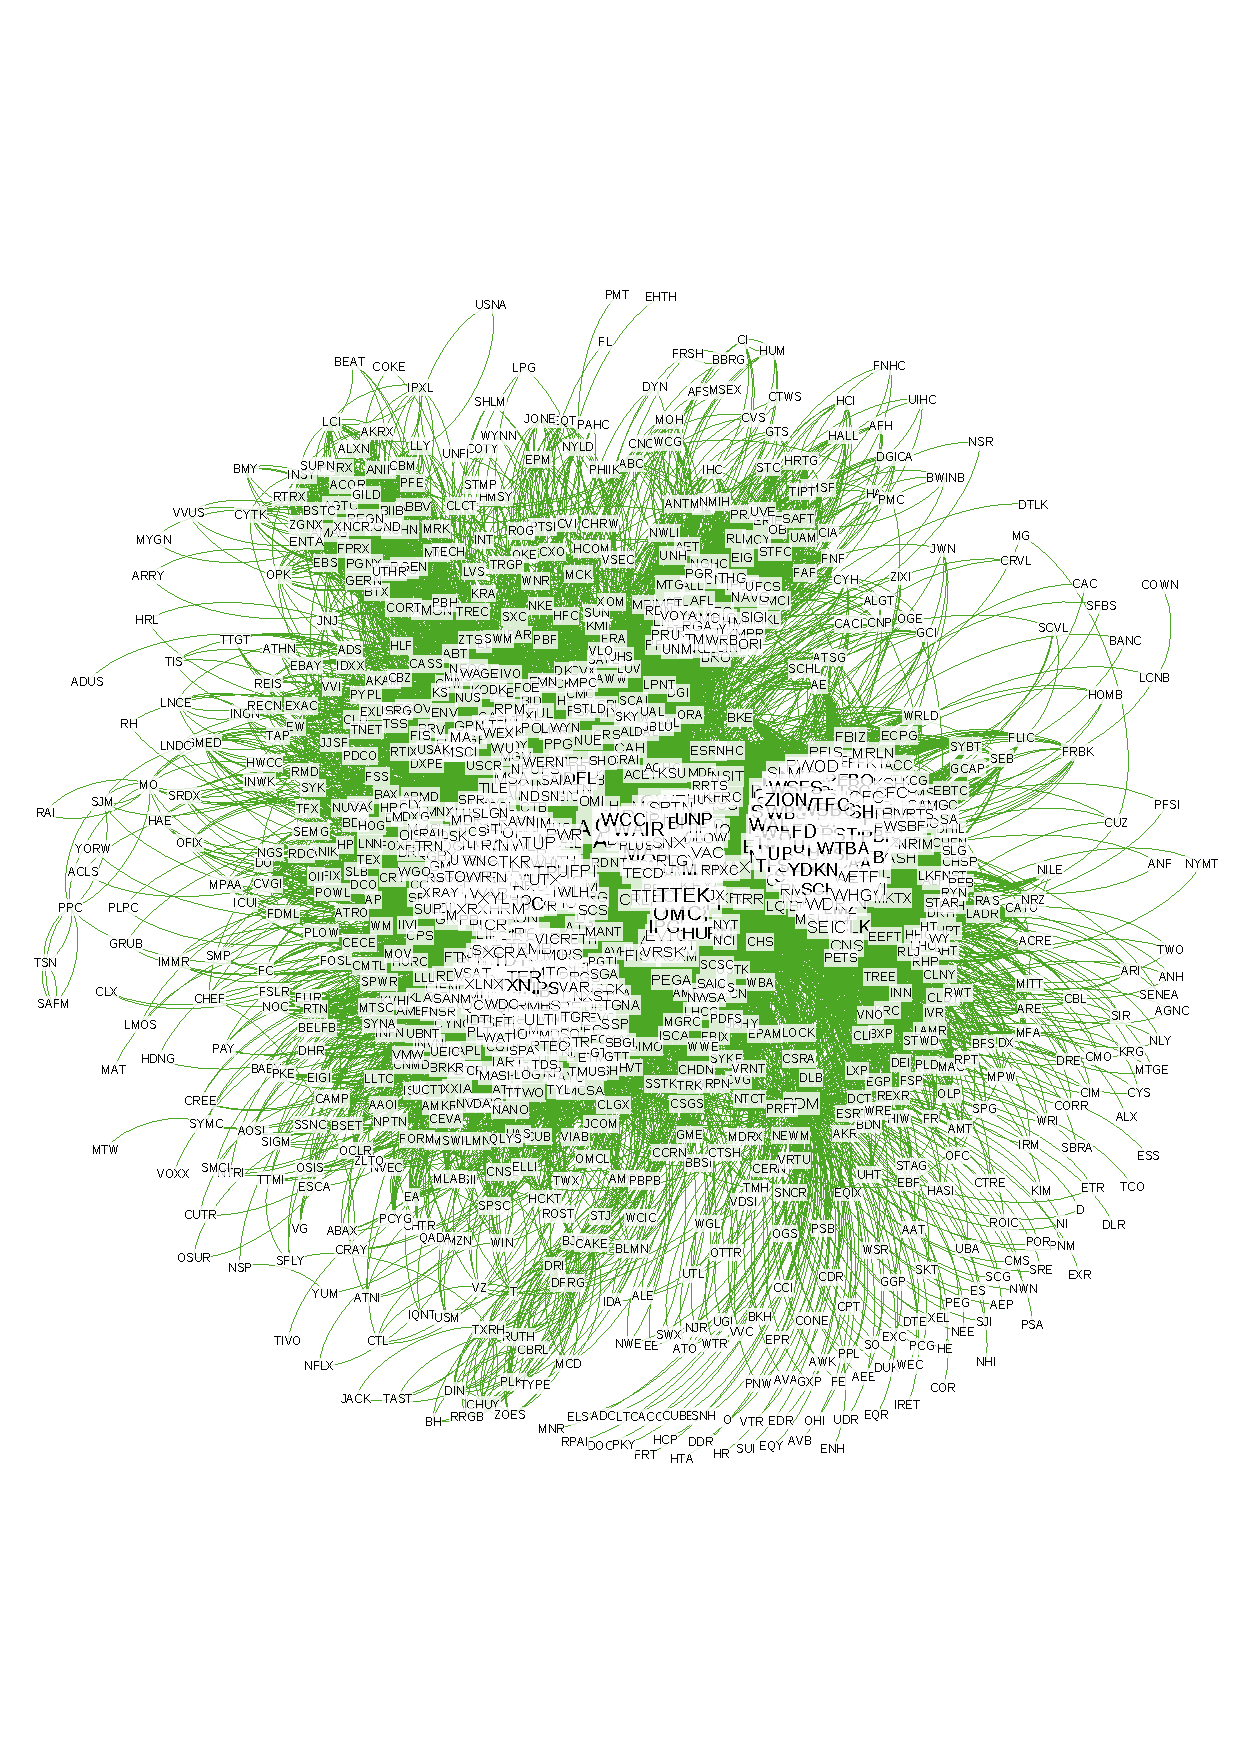
\includegraphics[width=14cm]{Graph_01}
	\end{center}
	\caption{Visualisation of the directed-unweighted stock price return network. The stock codes are nodes and the clockwise rotations of edges are directions.}
	\label{fig:Graph_01}
\end{figure}

It is obvious that the larger values assigned to $\theta_{EIO}$ and $\theta_{corr}$, the more significant will be for the weights and directions of the remaining edges. But if the network becomes too sparse, it can not be strongly or even weakly connected and there would be many independent cliques, hence the network becomes too inefficient to be a senseful network. As a result, this paper selects the threshold-value-pair $\{\theta_{EIO}=0.292, \theta_{corr}=0.379\}$ to construct a directed-unweighted network and a directed-weighted network for the 2016 US stock market. Figure~\ref{fig:Graph_01} shows the visualisation of the directed-unweighted stock network.

\section{Analysis of the directed-unweighted stock network}
A directed WS small-world network and a directed ER random network with the same number of nodes and edges with the stock directed-unweighted network are generated according to algorithms~\ref{alg:smallworld} and \ref{alg:random}. Table~\ref{tab:three} compares the main topological properties of the three networks, which will be discussed together with some other measures in the following sections.

\begin{table}
	\begin{center}
		\begin{tabular}{r|c|c|c}\hline\hline
			\textbf{Directed networks}&\textbf{Stock price return}&\textbf{WS small-world}&\textbf{ER random}\\\hline
			Number of nodes&1418&1418&1418\\
			%Number of edges&102051&102088&102097\\
			Number of edges&102051&102051&102051\\
			Out-degree distribution&Power-law&Normal&Normal\\
			%Average out-degrees&143.94&143.99&144.00\\
			Average out-degrees&143.94&143.94&143.94\\
			Average path length&2.775&2.005&1.973\\
			Clustering coefficient&0.4675&0.1367&0.05105\\
			Global efficiency&0.2563&0.5161&0.5216\\
			Local efficiency&0.6276&0.5027&0.4456\\
			Assortativity&0.02004&-0.002180&0.001452\\
			\hline\hline
		\end{tabular}
	\end{center}
	\caption{Main properties of stock network, small-world network, and random network}\label{tab:three}
\end{table}

\subsection{Power-law distribution}
\begin{figure}
	\subfloat[Empirical out-degree distribution]{%
		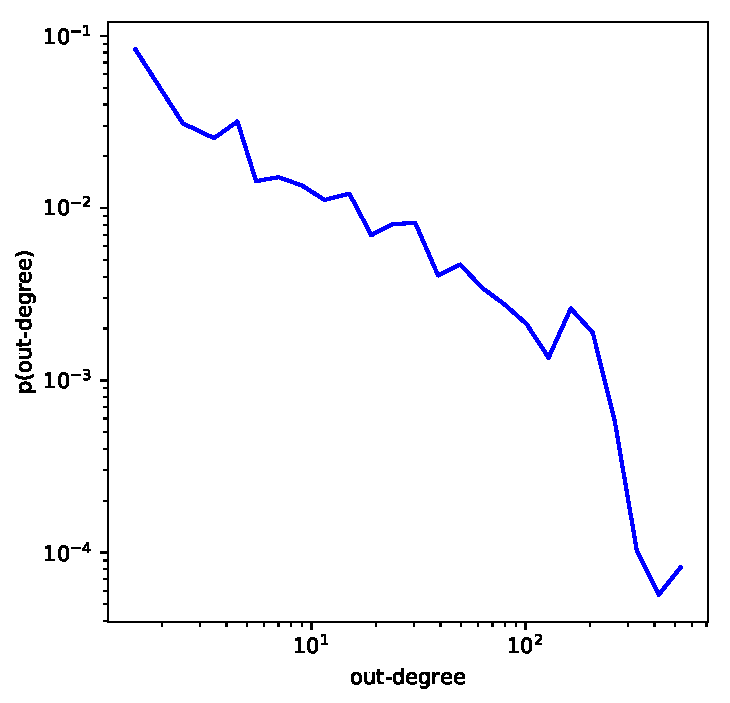
\includegraphics[width=0.46\textwidth]{G_out_degree_distribution_square}%
		\label{fig:G_out_degree_distribution_square}%
	}%
	\hfill%
	\subfloat[CCDF and power-law fit]{%
		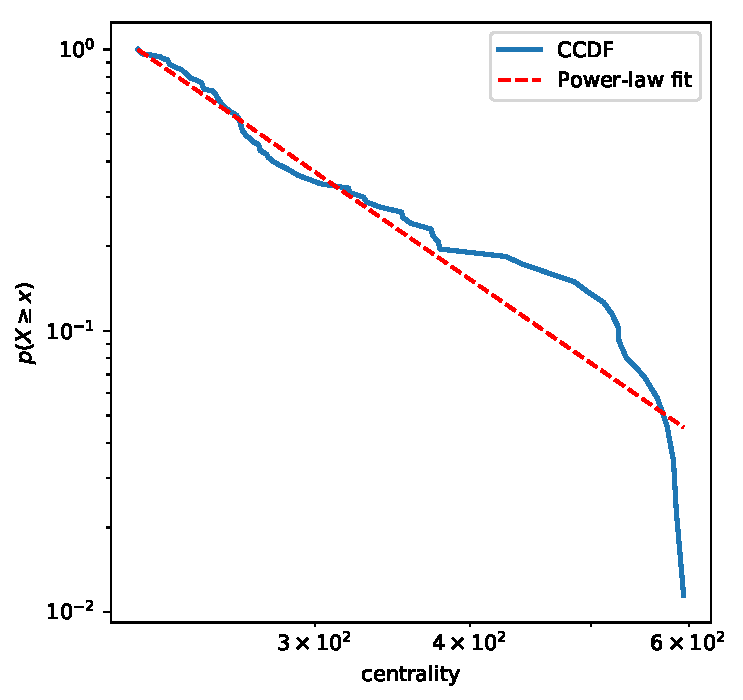
\includegraphics[width=0.465\textwidth]{out_degree_log_fit_square}%
		\label{fig:out_degree_log_fit_square}%
	}%
	\caption{Out-degree distribution of directed stock price return network} \label{fig:outdegreedistribution}
\end{figure}

\begin{figure} % P-P SW
	\centering
	\subfloat[Empirical out-degree distribution]{
		\label{subfig:G_sw_out_degree_distribution}
		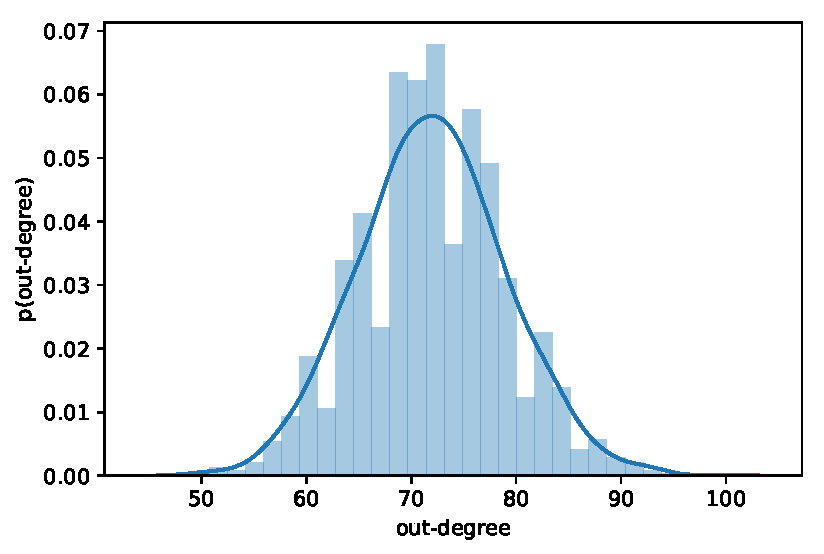
\includegraphics[width=12cm]{G_sw_out_degree_distribution} }
	
	\subfloat[P-P plot]{
		\label{subfig:G_ws_mat_prob_plot}
		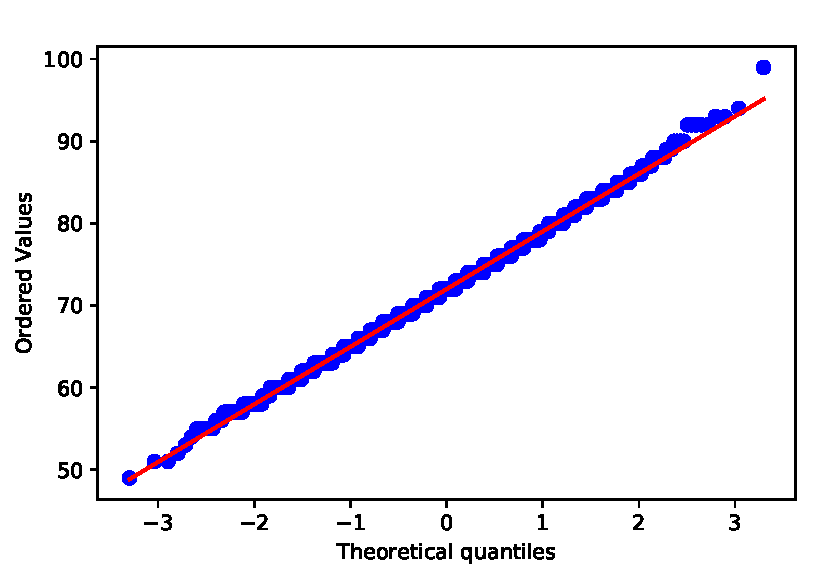
\includegraphics[width=12cm]{G_ws_mat_prob_plot} }
	
	\caption{Out-degree distribution and P-P plot of small-world network}
	\label{fig:distributionsm}
\end{figure}

\begin{figure} % P-P rd
	\centering
	\subfloat[Empirical out-degree distribution]{
		\label{subfig:G_rd_out_degree_distribution}
		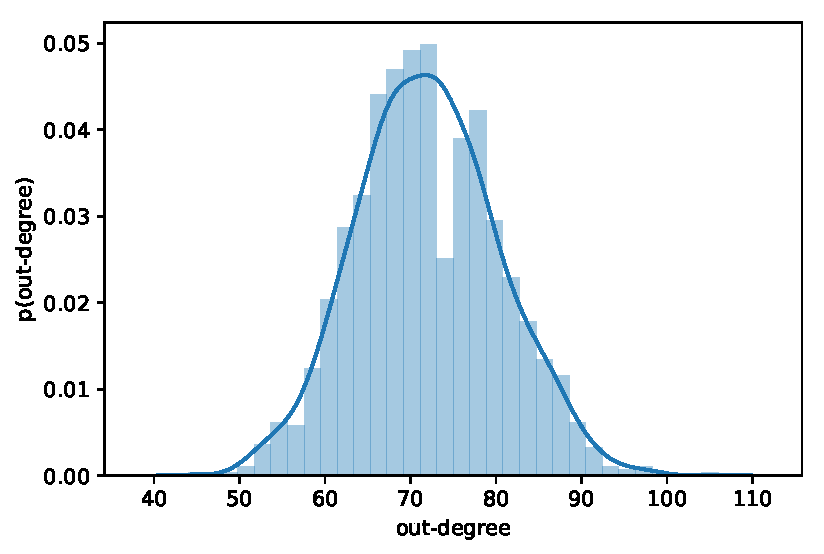
\includegraphics[width=12cm]{G_rd_out_degree_distribution} }
	
	\subfloat[P-P plot]{
		\label{subfig:G_rd_prob_plot}
		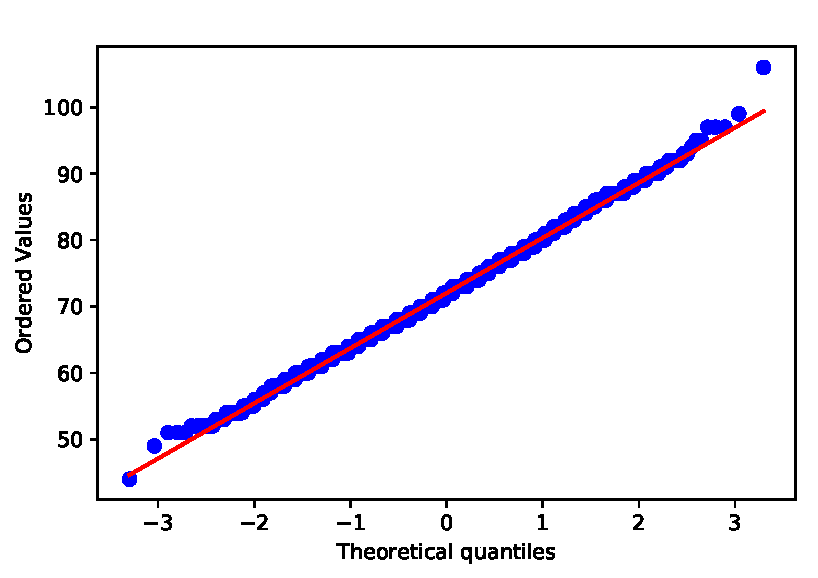
\includegraphics[width=12cm]{G_rd_prob_plot} }
	
	\caption{Out-degree distribution and P-P plot of random network}
	\label{fig:distributionrd}
\end{figure}

According to the table~\ref{tab:three}, the values of average out-degrees of directed stock network, WS small-world network and ER random network are exactly the same due to the identical numbers of nodes and edges, but in terms of the distributions of out-degrees, stock network is totally different from the others. 

The distribution and P-P plots in figures~\ref{fig:distributionsm} and \ref{fig:distributionrd} show clearly that the out-degree distributions of WS small-world network and ER random network fitted nicely to the normal distribution, because most degrees of nodes fall in the middle range, especially in the P-P plots, the sample data points are basically on the diagonal representing the theoretical normal distribution for both WS small-world network and ER random network. Nonetheless, figure~\ref{fig:G_out_degree_distribution_square} illustrates that for the stock price return network, only a few number of nodes show higher out-degree, while most nodes are at the positions of low out-degree level. Statistical result shows the distribution of the directed stock price return network follows power-law distribution with the exponent of $4.057$.

The discovered power-law distribution property reveals that in the aspect of degree the directed stock network shows the continuity with conventional undirected stock networks in previous studies. Therefore in general, most of the nodes have a small degree while a few modes have a higher degree for both directed and undirected stock networks.

\subsection{Small-world property}
Previous researches upon undirected stock networks have argued that they have small-world topologies. Such feature is also applied to the directed WS small-world network and ER random network, for the average path lengths of around $2$, indicating that if we take any node in the network, it can be expected to reach any other nodes just through one node as the medium. For the directed stock network, the expectation number of medium nodes is $1.775$, which can be also treated as a small number for network connectedness.

On the other hand, the global efficiency of the benchmarking networks are slightly higher than $1/l_G$ which are both around $0.5$. It means that in physical terms the flow of information in these two networks is efficient, which is the behaviour of small-world networks. While as for the directed stock network, its global efficiency is less than $1/l_G$ which is $0.36$. In essence, like directed WS small-world and ER random networks, directed stock network also has the small-world properties to some degree, while it is not efficient to exchange information across the network in the global scale.

\subsection{Clustering feature}
The directed ER random network shows no clustering feature because its clustering coefficient is close to zero ($0.05105$). For the directed WS small-world network, its clustering coefficient of $0.1367$ shows slight clustering feature. While for the directed stock network, its clustering coefficient of 0.4675 is much higher, which shows an significant clustering feature. The indicator of local efficiency also support this conclusion because it reveals the neighbours of a node in the directed stock network are more efficient when conduct information than the other two benchmarking networks, therefore the nodes in the stock network tend to cluster together in higher degree.

The assortativity values for the three networks are all non-significant, for the two benchmarking networks this is corresponding to the aforementioned non-clustering feature and the normal distribution of degrees. However, for the stock network, the incredibly low assortativity together with the aforementioned power-law distribution of degrees indicate that the nodes in this network tend to connect to other nodes with high degrees.

\subsection{Community structure of the directed-unweighted stock network}
The larger value of clustering coefficient for stock network than the other two networks indicating that the nodes in stock network tend to cluster together. Therefore, communities of stock network will be identified implementing the \textit{algorithm~\ref{alg:communitydetection}} for directed networks in this section. According to the composition of industrial sectors of each community, as figure~\ref{fig:community_sector_stacked} shows, the following five communities are identified: (1) Production (2) Finance (3) Livelihood (4) Insurance and chemical products (5) Utilities and financial vehicles.

The communities of production (purple) and livelihood (blue) are sparsely distributed while there are some large-sized nodes acting as hubs of the overall network. The hubs not only connect to the nodes of same communities, but also the externals. These two communities are partially intertwined due to the high relevancy of production industry and livelihood industry. 

Unlike the above two communities, it can be seen from figure~\ref{fig:community_graph} that the community of finance (green) is decentralised, i.e., there is no obvious hubs and the degrees of each node distribute evenly. It also has a very dense structure, connected closely inside and completely exclusive from other nodes or communities. This means the co-movements among financial stocks are incredibly strong and economically they rely tightly to each other.

The other two communities are more interesting because of their peculiar structural features. Every industrial sectors of individual stocks in community are identified to investigate the properties of the community of insurance and chemical products (yellow). As figure~\ref{fig:community_4} illustrates and through the investigation, almost all firms in the upper and lower clusters are in the sectors of "chemical products" and "insurance carriers and related activities" respectively, while firms between the two big clusters, like "MCK" (McKesson) and "CAH" (Cardinal Health), are large medical supplier, pharmaceutical and heathcare service companies with high out-degrees to both of the two clusters. Apart from that, there are also a considerable number of links from the nodes in upper cluster to the hubs of chemical companies. Thus, it is reasonable to infer that the prices of medicines have significant influence to medical insurance industry, additionally the purchases of chemical products of pharmaceutical firms and the sales of chemical products have made pharmaceutical and chemical companies influence to each other.

Another investigation towards the community of utilities and financial vehicles (orange) is conducted by the same measure. As figure~\ref{fig:community_5} illustrates, there is only one huge hub (PDM) which is the company "Piedmont Office Realty Trust" among the whole community while all the others are one-degree nodes located remotely. There are more links from the hub to the rest than the opposite direction, and also the weights of the former links are generally higher. The hub, "Piedmont Office Realty Trust", is a real estate investment trust company, and the rest in the community contains 59 "funds, trusts, and other financial vehicles" firms and 44 "utilities" firms. For a big realty trust enterprise, demand for financial trust business is extremely high, and its successes of investments upon real estates will promote the development of utilities companies. It depicts that the major realty trust enterprise alone has significant influence to all of these financial trust and utilities companies.

\begin{figure}
	\begin{center}
		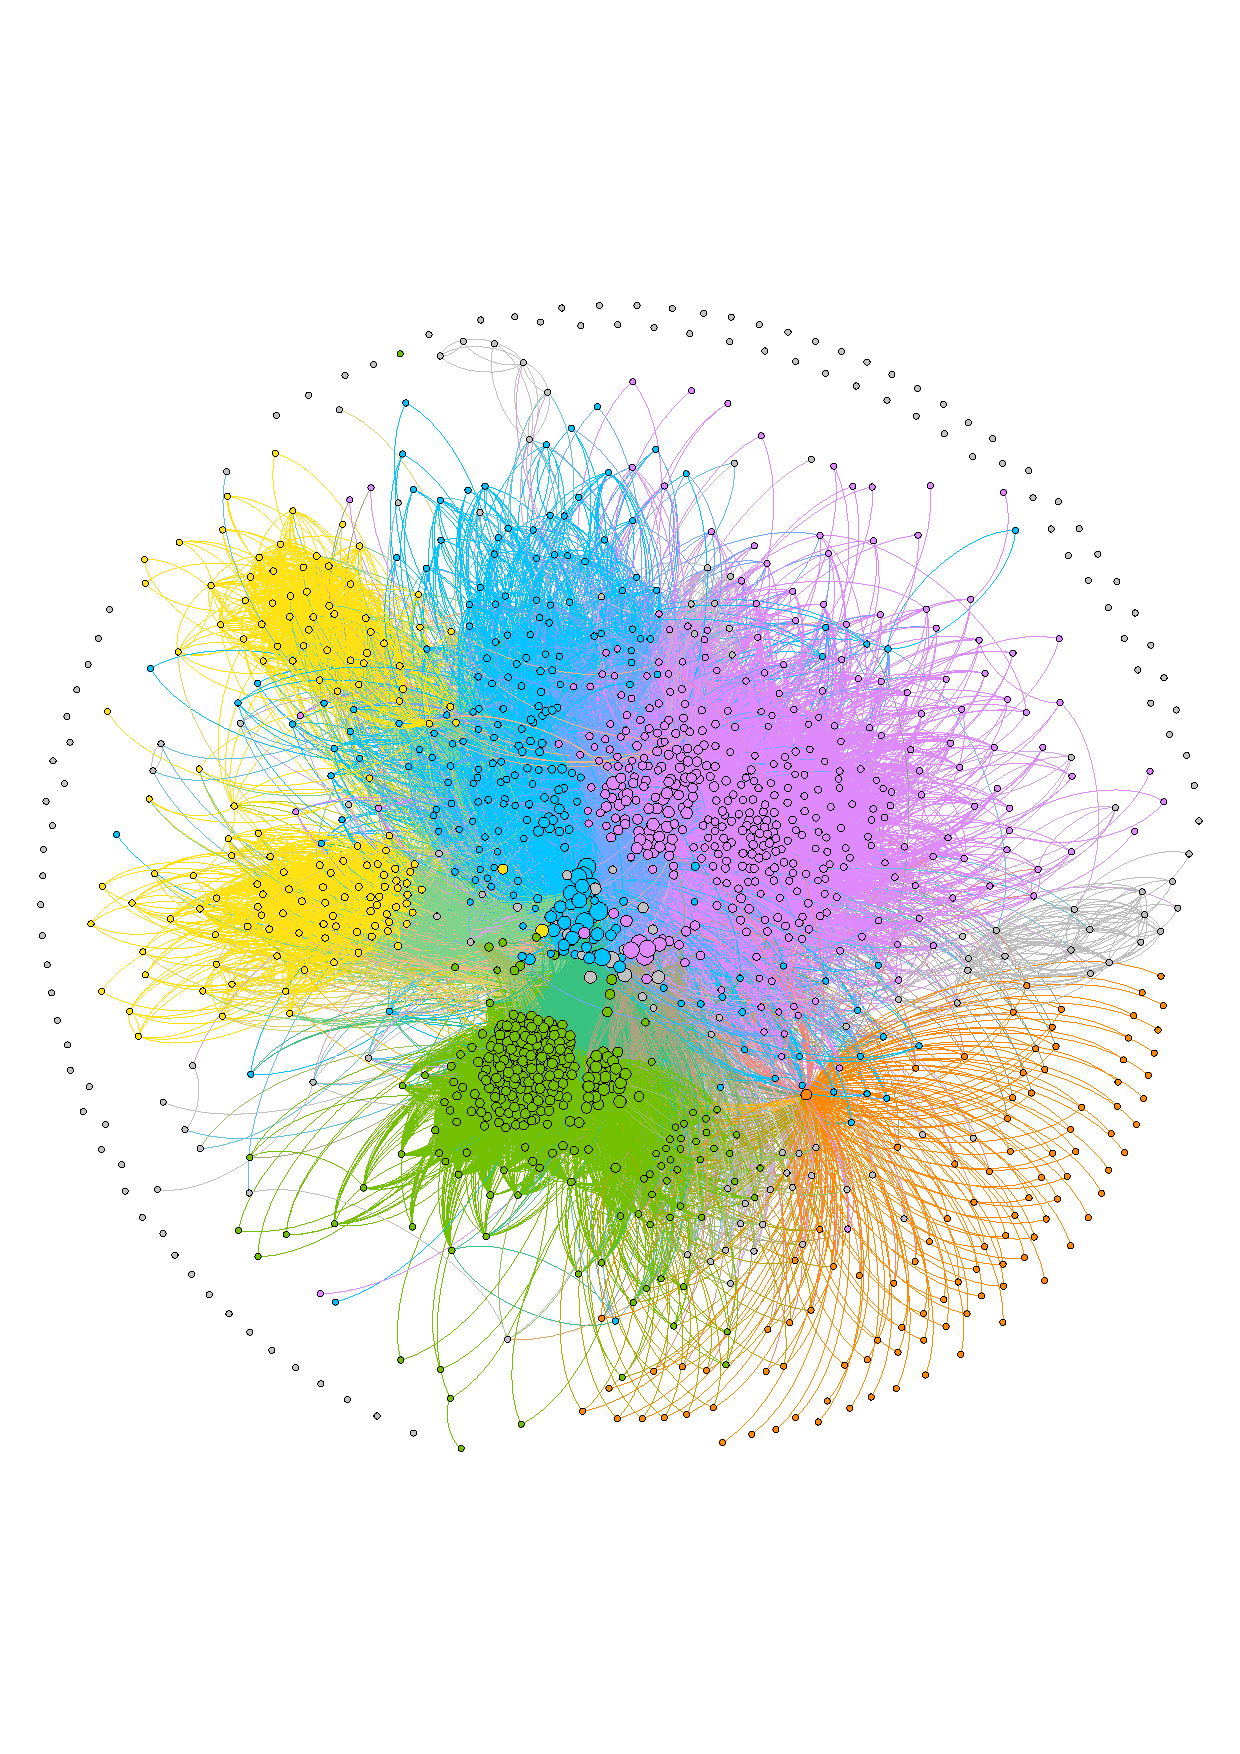
\includegraphics[width=14cm]{community_graph}
	\end{center}
	\caption{Community structure of the 2016 US stock price return network. Five distinct communities are detected represented by different colours of nodes. The direction of edge is  clockwise. The size of nodes and thickness of edges are related to the value of degrees and weights. The grey nodes do not belong to any communities and most of them have zero degree.}%use gephi
	\label{fig:community_graph}
\end{figure}

\begin{figure} % 各个单独的群落
	\subfloat[Production]{%
		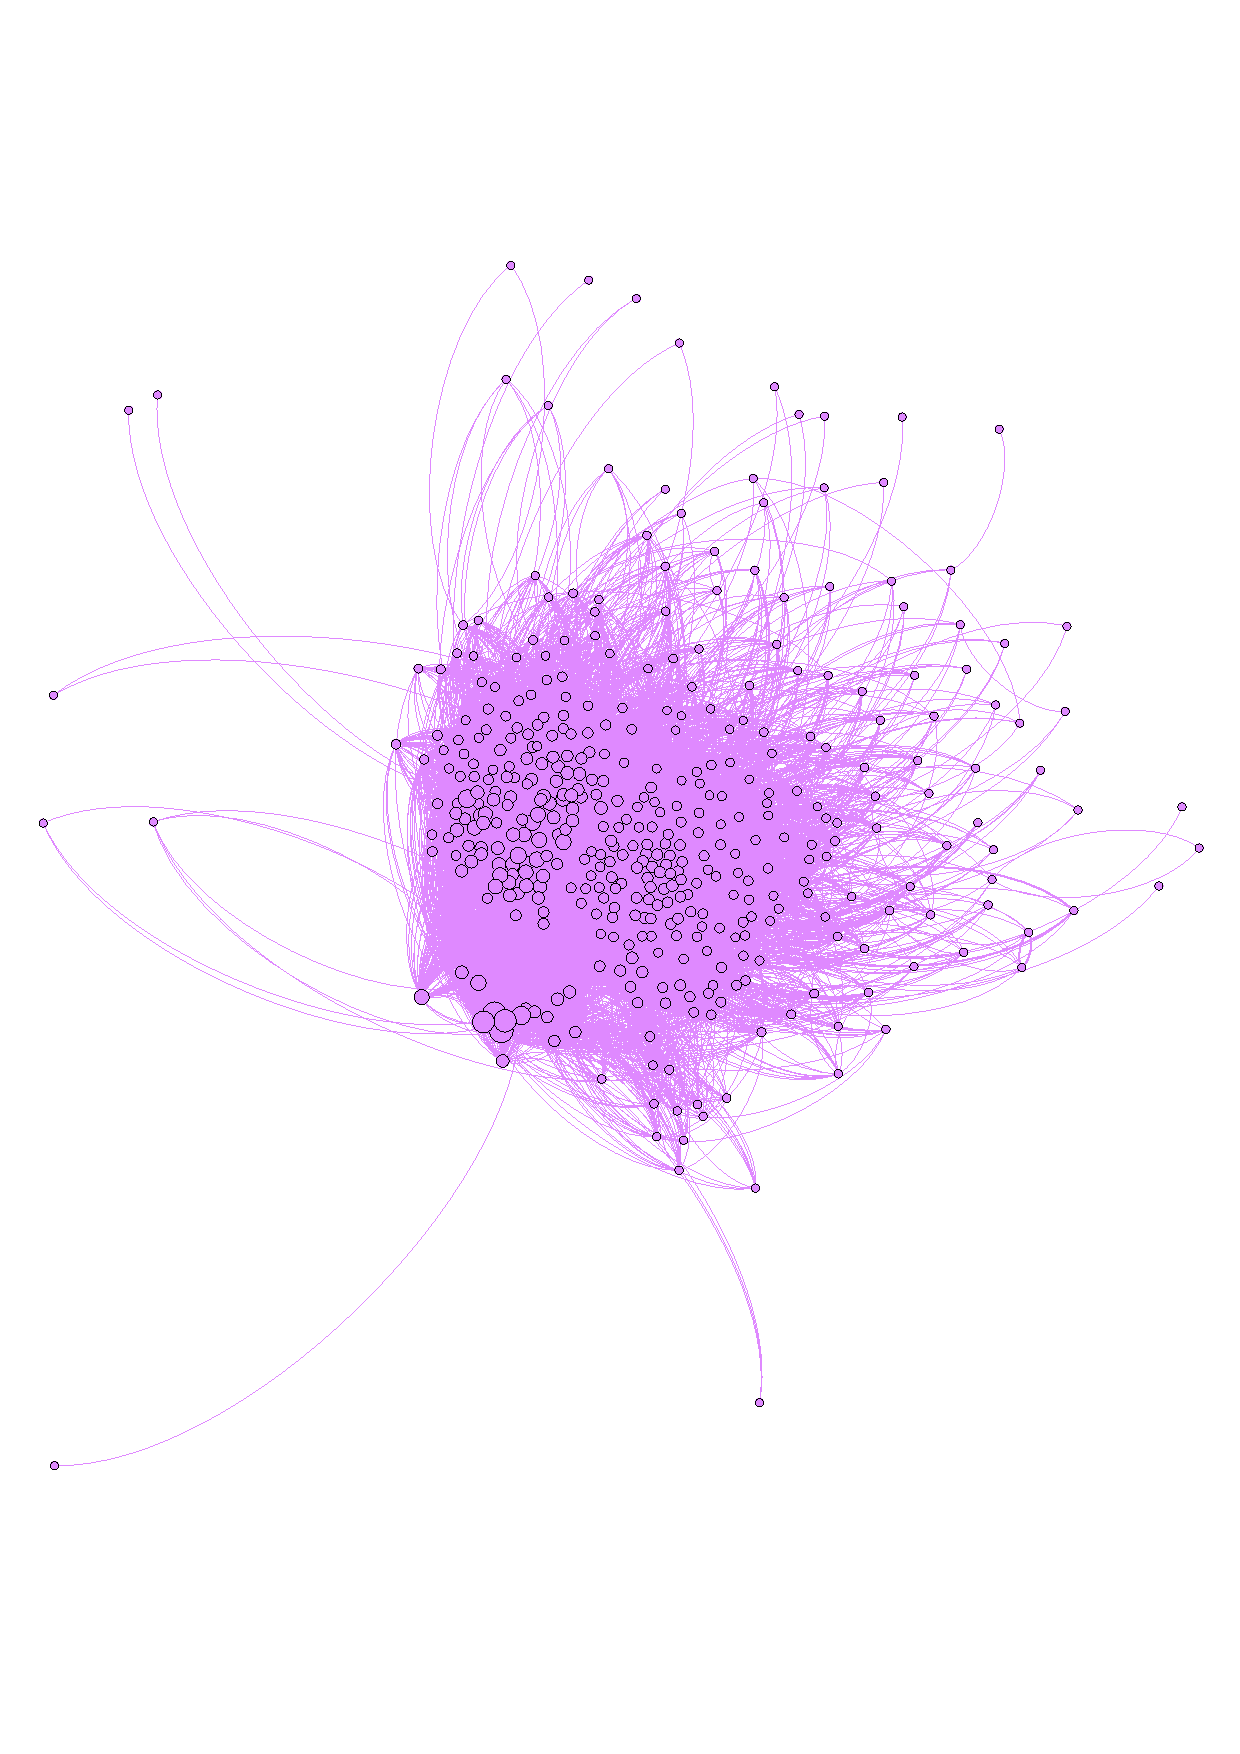
\includegraphics[width=0.45\textwidth]{community_1}%
		\label{fig:community_1}%
	}%
	\hfill%
	\subfloat[Finance]{%
		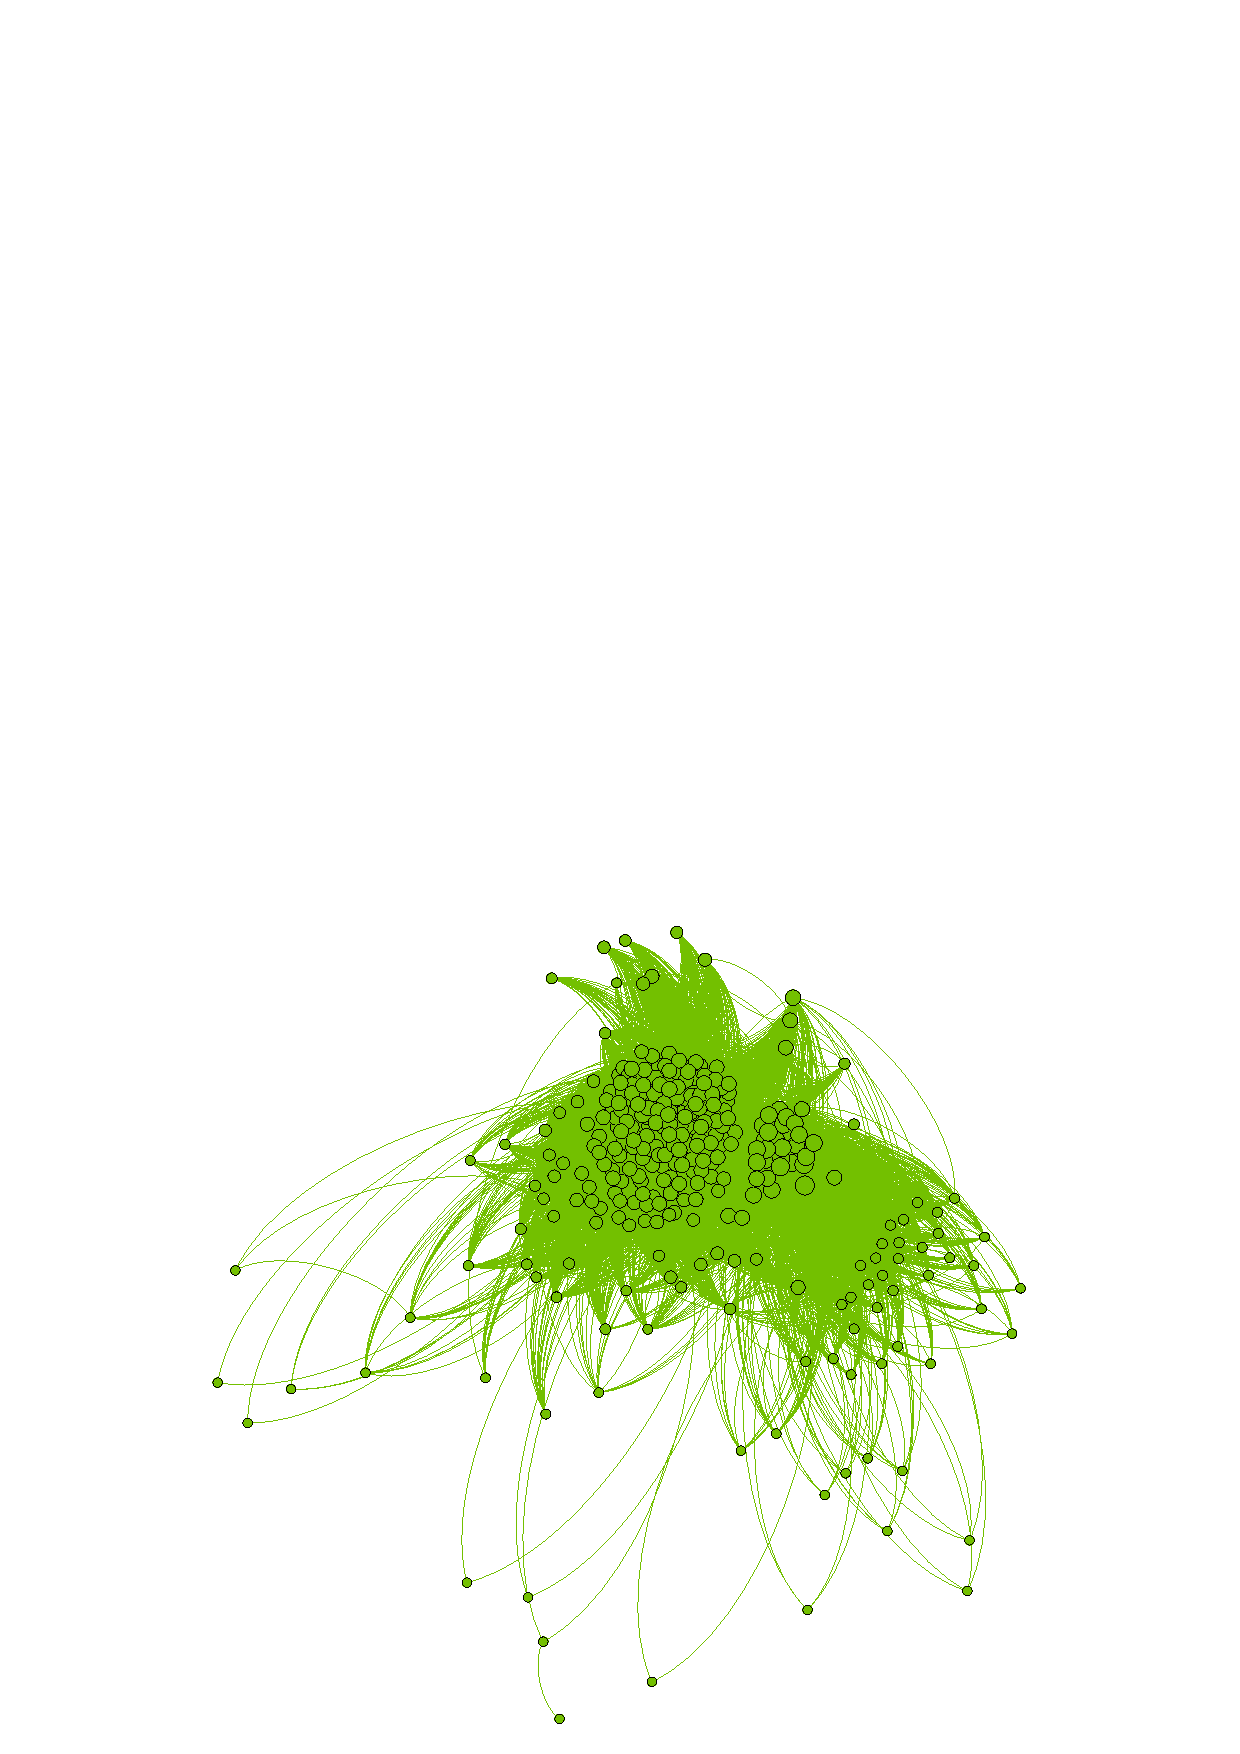
\includegraphics[width=0.45\textwidth]{community_2}%
		\label{fig:community_2}%
	}%
	\hfill%
	\subfloat[Livelihood]{%
		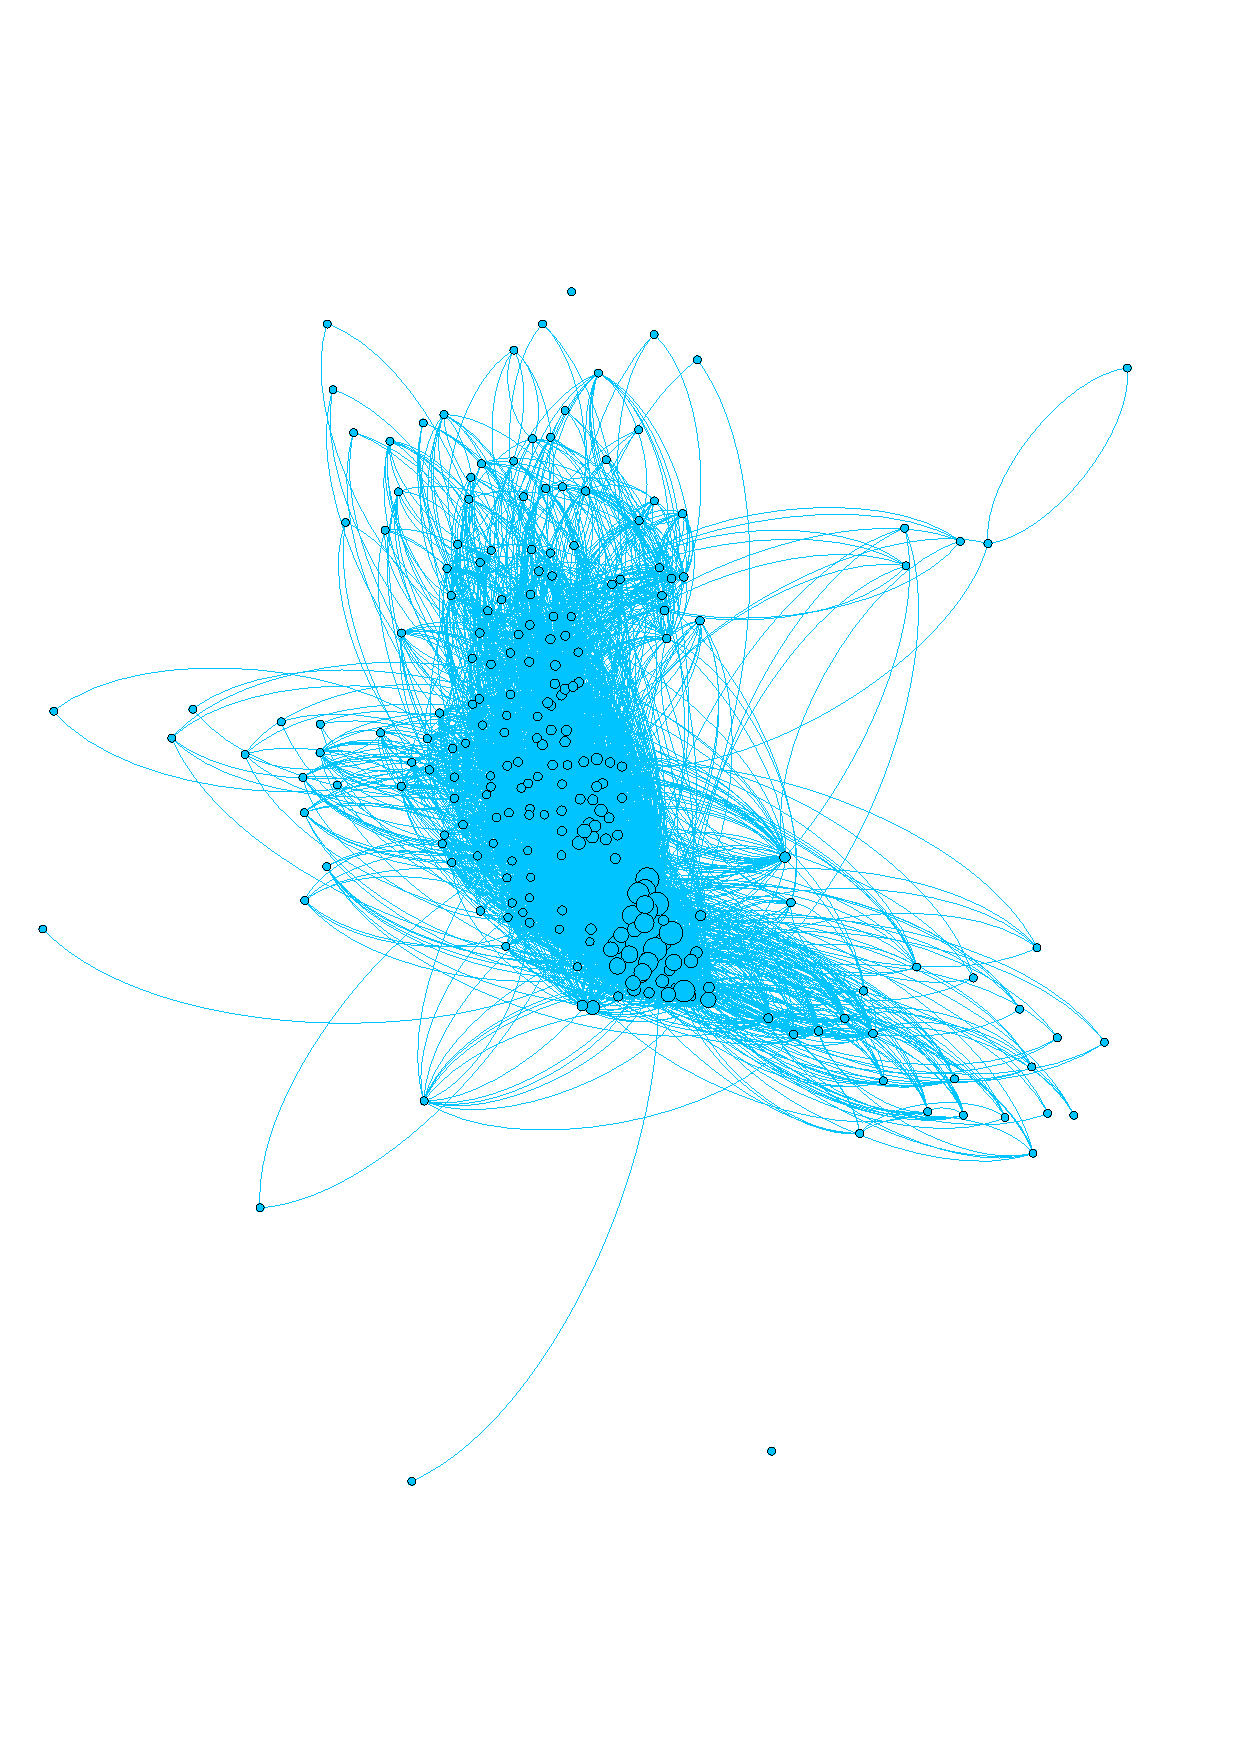
\includegraphics[width=0.45\textwidth]{community_3}%
		\label{fig:community_3}%
	}%
	\hfill%
	\subfloat[Insurance and chemical products]{%
		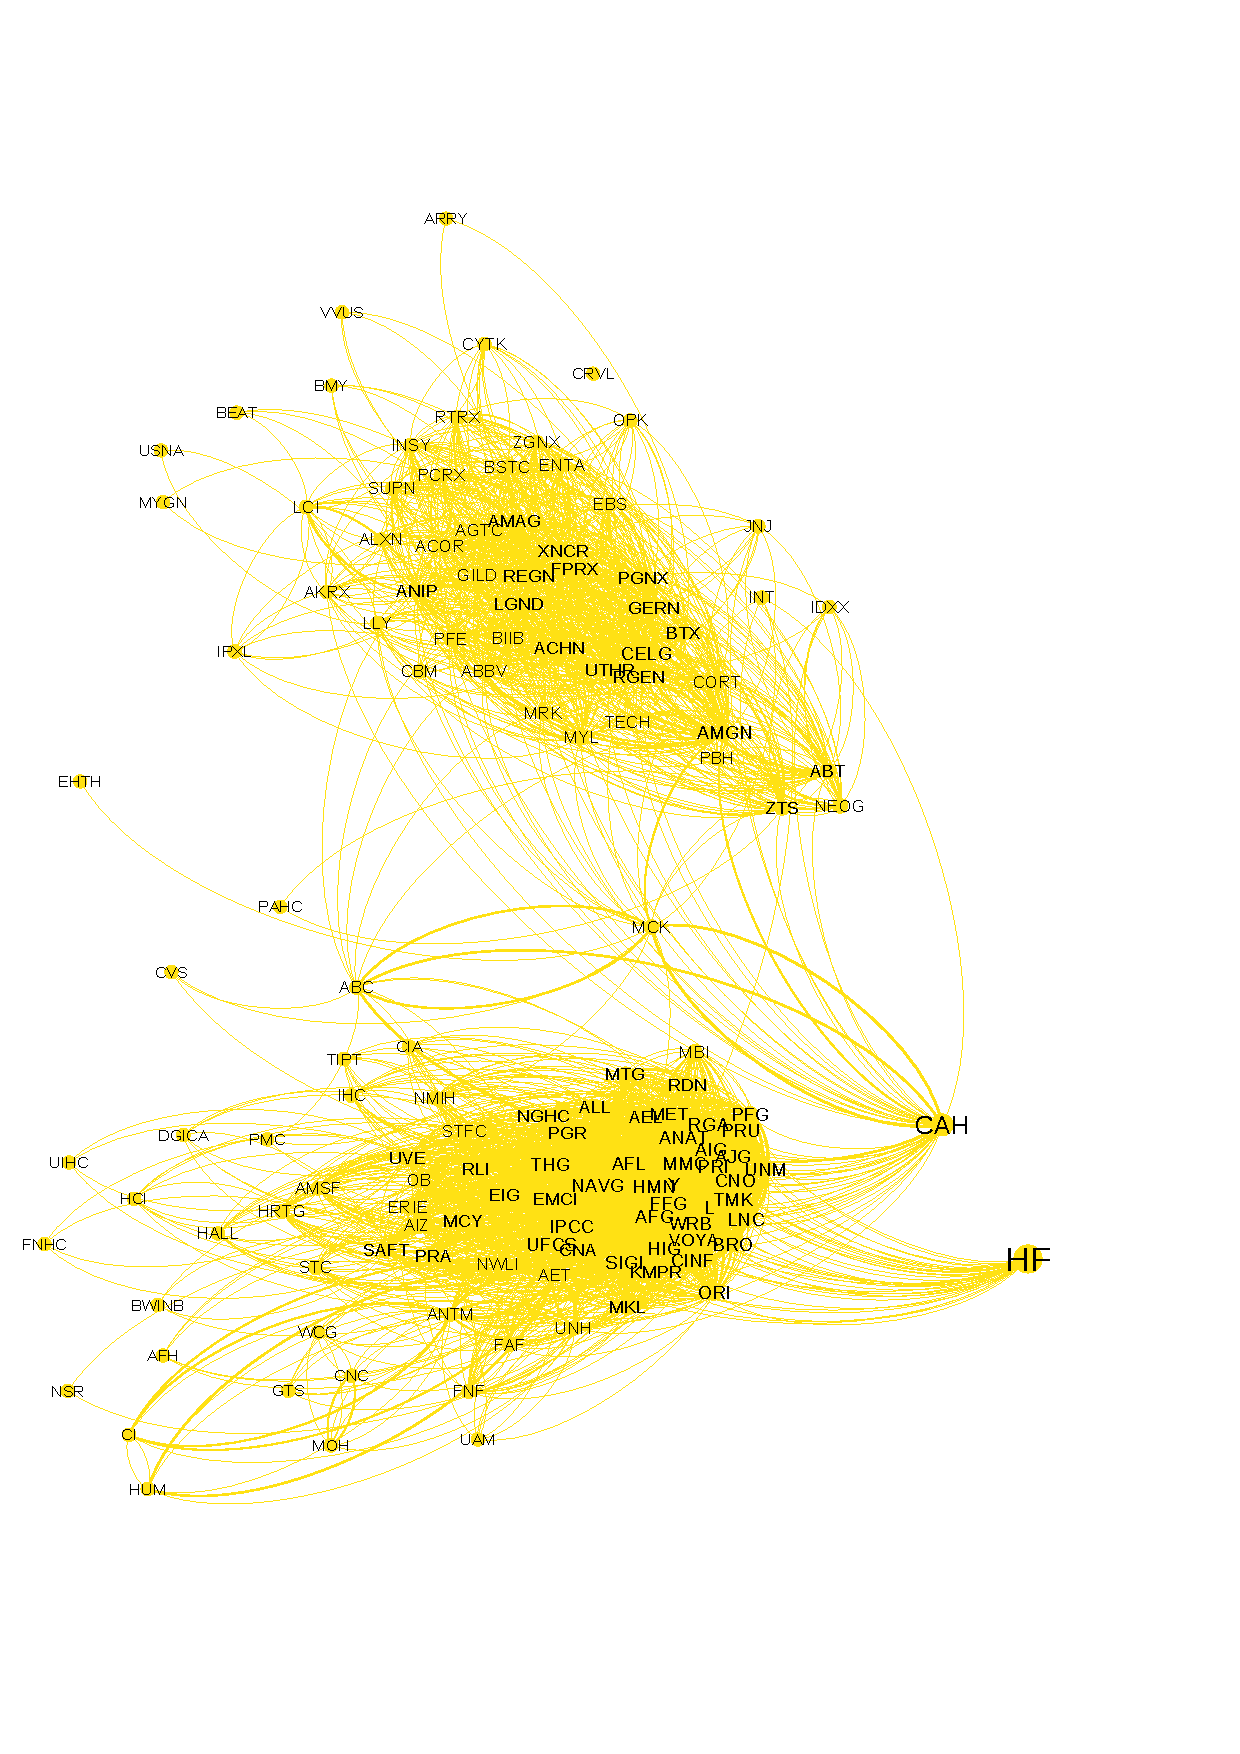
\includegraphics[width=0.45\textwidth]{community_4}%
		\label{fig:community_4}%
	}%
	\hfill%
	\subfloat[Utilities and financial vehicles]{%
		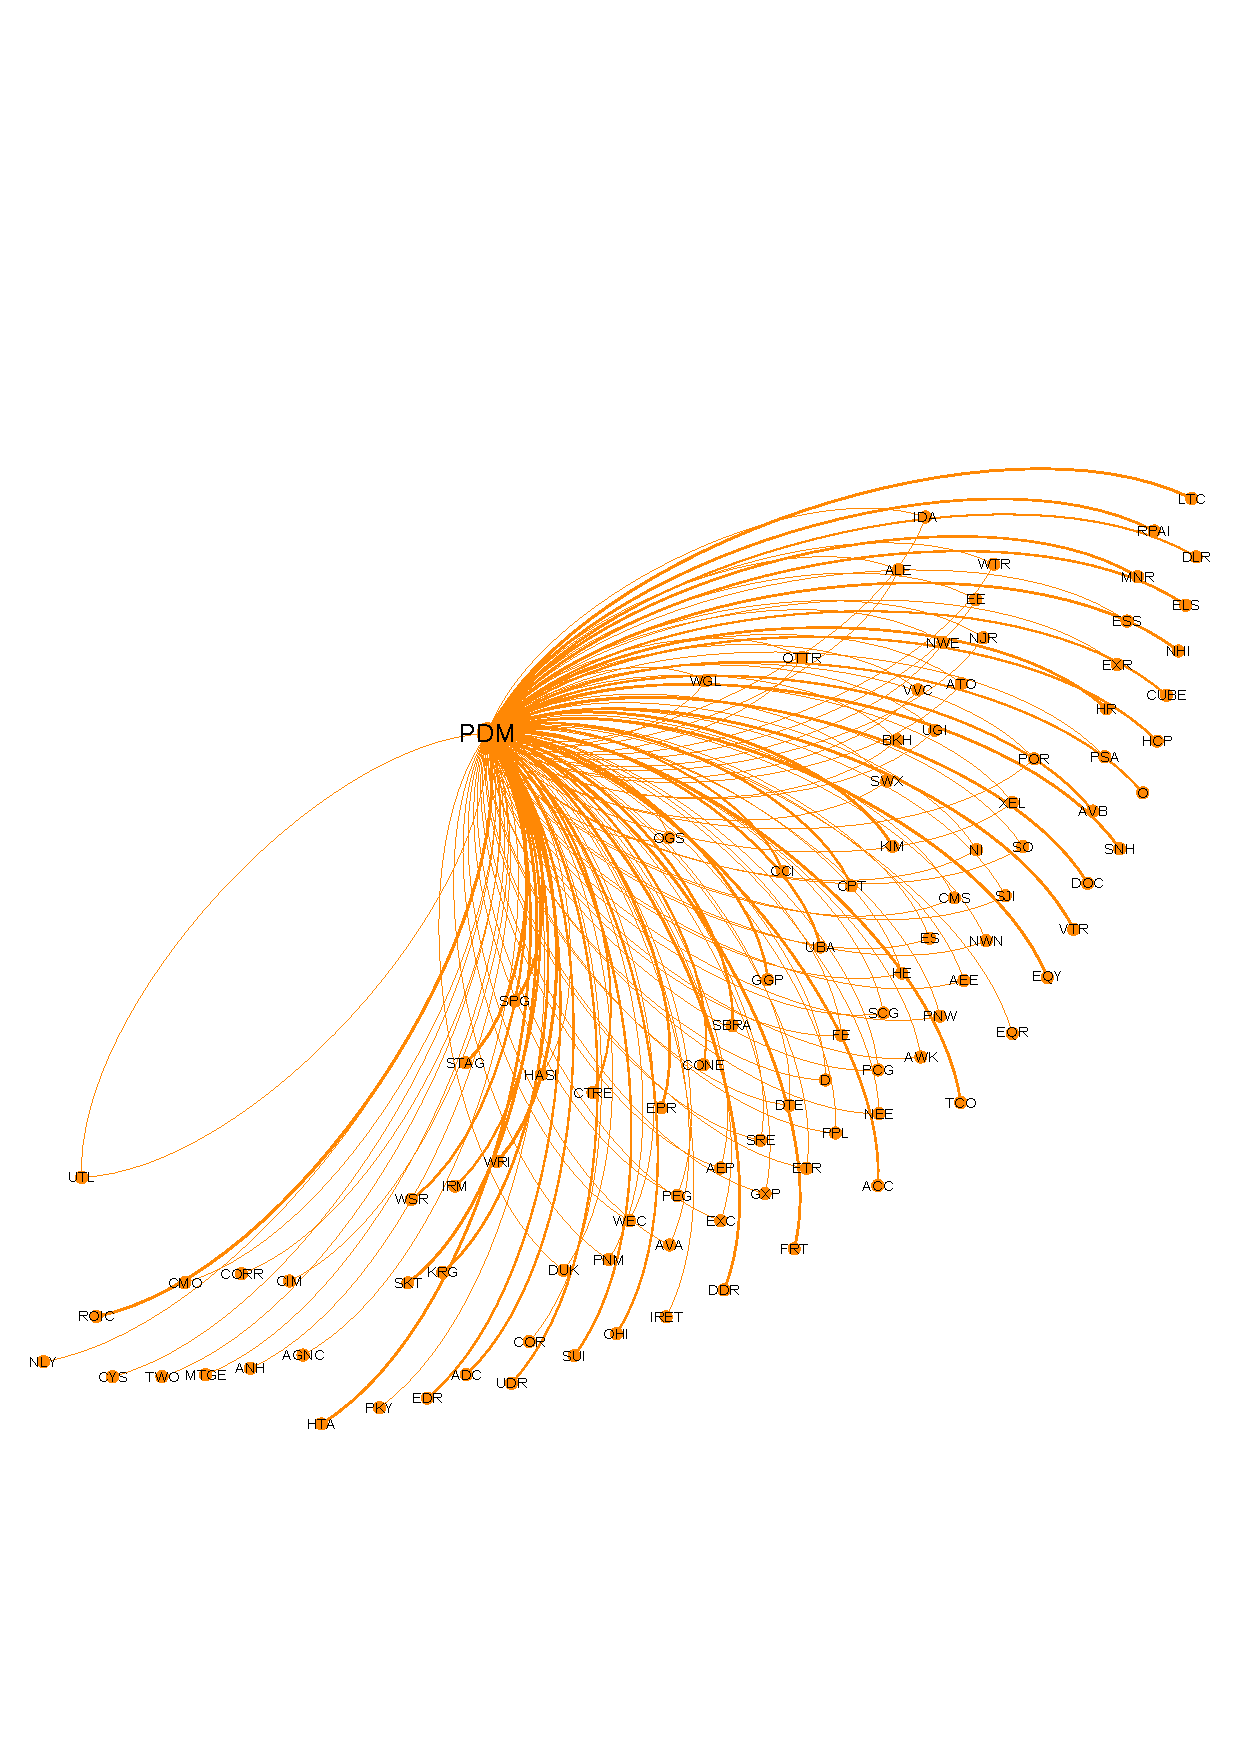
\includegraphics[width=0.45\textwidth]{community_5}%
		\label{fig:community_5}%
	}%
	\caption{Community sole views of the directed stock network. Stock tickers are displayed for the sparsely distributed communities.} \label{fig:distinctcommunities}
\end{figure}

\begin{figure} % 群落的行业柱形图
	\begin{center}
		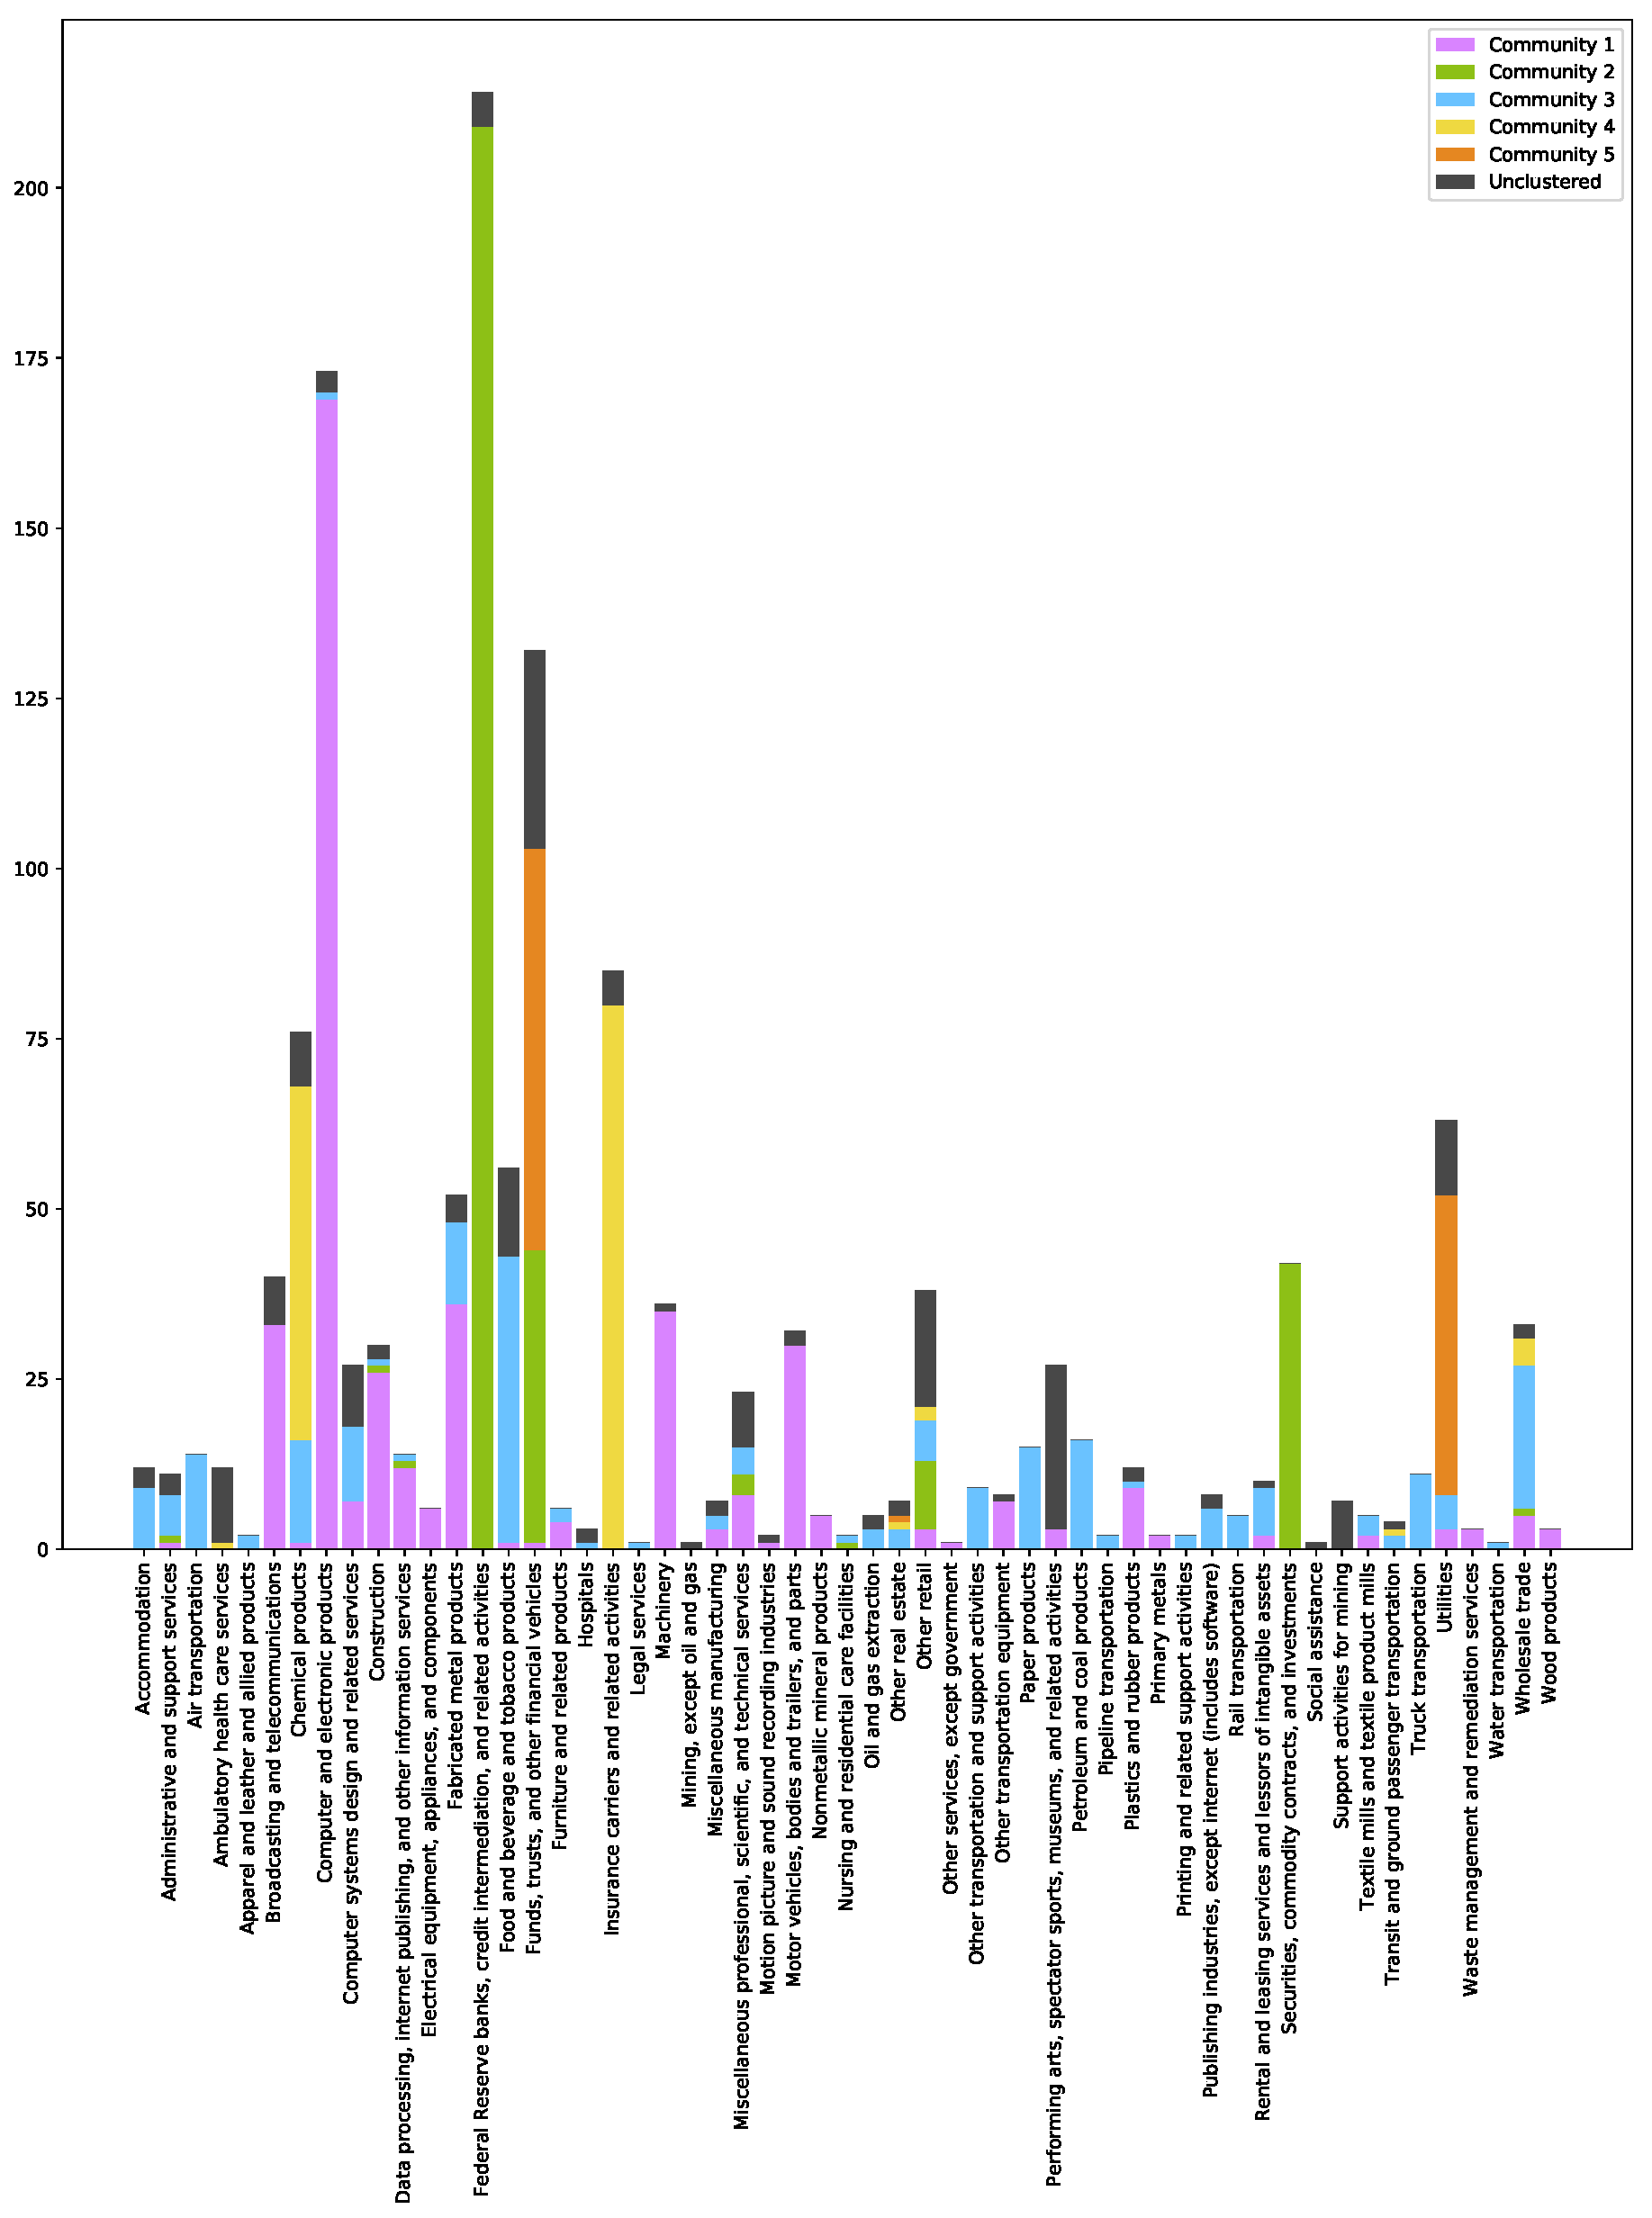
\includegraphics[width=15cm]{community_sector_stacked}
	\end{center}
	\caption{Stacked bar chart about the distribution of communities upon industrial sectors. Colours of stacks correspond to the colours of communities in figure~\ref{fig:community_graph} and figure~\ref{fig:distinctcommunities}, except the black stack indicating the nodes not belong to any communities. Sectors are arranged alphabetically.}
	\label{fig:community_sector_stacked}
\end{figure}

\iffalse
\begin{figure}
	\begin{center}
		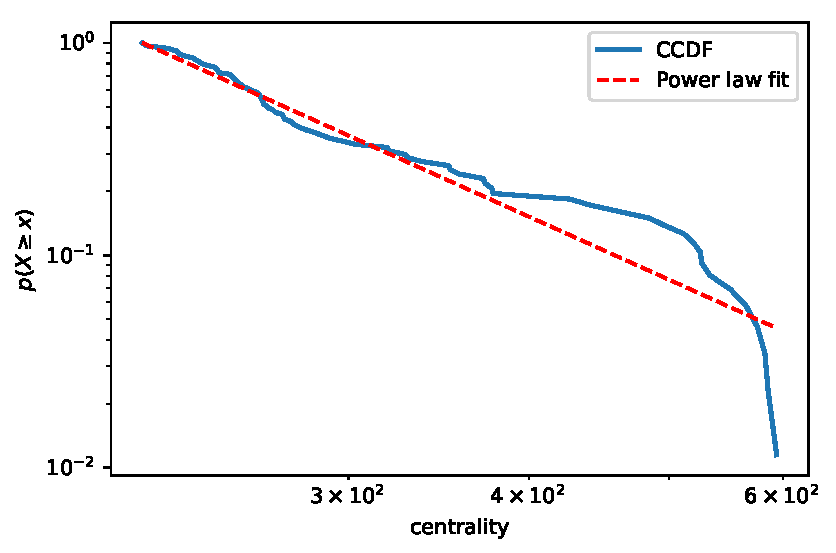
\includegraphics[width=15cm]{out_degree_log_fit}
	\end{center}
	\caption{Amounts of edges per EIO-threshold and correlation-coefficient-threshold}
	\label{fig:out_degree_log_fit}
\end{figure}
\fi

\section{Analysis of the directed-weighted stock network}
A directed-weighted stock network is generated by adding the correlation coefficients in the matrix \textbf{C} as weights to each existing directed edges from the directed-unweighted stock network. As the weighted form of the directed stock network that discussed in previous sections, this section will only focus on its features about the weights.
\subsection{Topological properties on weighted networks}
A conventional undirected-weight network is constructed independently and through the threshold of correlation coefficient we can adjust the number of undirected edges remain. When converting an undirected network to directed network, the number of edges are doubled because each undirected links are generated into two directed links with opposite directions for remaining original network topological features unchanged. Same reason is applied for constructing the conventional undirected-weighted stock network with equivalent topologies with the directed stock network. Hence, table~\ref{fig:topology_weighted} compares the topological properties between them.

\iffalse
\begin{table}
	\begin{center}
		\begin{tabular}{r|c}\hline\hline
			&Undirected stock network\\\hline
			Degree distribution & Power-law\\
			Average out-degrees & Power-law\\
			Average path length & 2.775\\
			Average strength & 42.31\\
			Average betweenness centrality & 0.0007464\\ % 0.0007464209710184614
			Weighted assortativity & 0.06138\\ % 0.06138005376924545
			Clustering coefficient & 0.4675\\
			Global efficiency & 0.2563\\
			Local efficiency & 0.6276\\
			Assortativity & 0.02004\\
			\hline\hline
		\end{tabular}
	\end{center}
	\caption{Main topologies of conventional stock price network}
	\label{tab:conventional}
\end{table}
\fi

\begin{table}
	\begin{center}
		\begin{tabular}{r|c|c}\hline\hline
			Weighted stock network&Directed&Undirected\\\hline
			Number of nodes & 1418 & 1418\\
			Number of edges & 102051 & 51037\\
			Strength distribution & Power-law & Power-law\\
			Average strength & 40.89 & 42.31\\ % 40.88927702272619
			Average betweenness centrality & 0.0007440 & 0.0007464\\
			Weighted assortativity & 0.1244 & 0.06138\\ % Assortativity with weight 0.12444731038165072
			\hline\hline
		\end{tabular}
	\end{center}
	\caption{Main topologies of weighted stock networks}\label{tab:weighted}
	\label{fig:topology_weighted}
\end{table}

Like directed-unweighted stock network, and also conventional weighted stock networks, the strength distribution of directed-weighted stock network follows power-law distribution. The average strength and betweenness centrality of the two weighted networks are close to each other. But interestingly, the directed-weighted stock network has significantly high assortativity other than directed-unweighted and conventional weighted networks. It reveals that in the researched stock networks, nodes tend to be connected with other nodes with similar strength values rather than degree values, which means stocks tend to have relationships with other stocks with similar fluctuation in stock price return. Therefore, correlation coefficient is an important factor for the behaviour of node connections.

\subsection{Analysis on the relationships between price return and betweenness centrality}
\begin{figure}
	\subfloat[Bivariate distribution beween betweenness centralities of nodes and cumulative sums of stock daily return. The returns are actually logarithmic returns therefore the accumulation of all daily logarithmic returns in an entire year equals to a corresponding yearly logarithmic return.]{%
		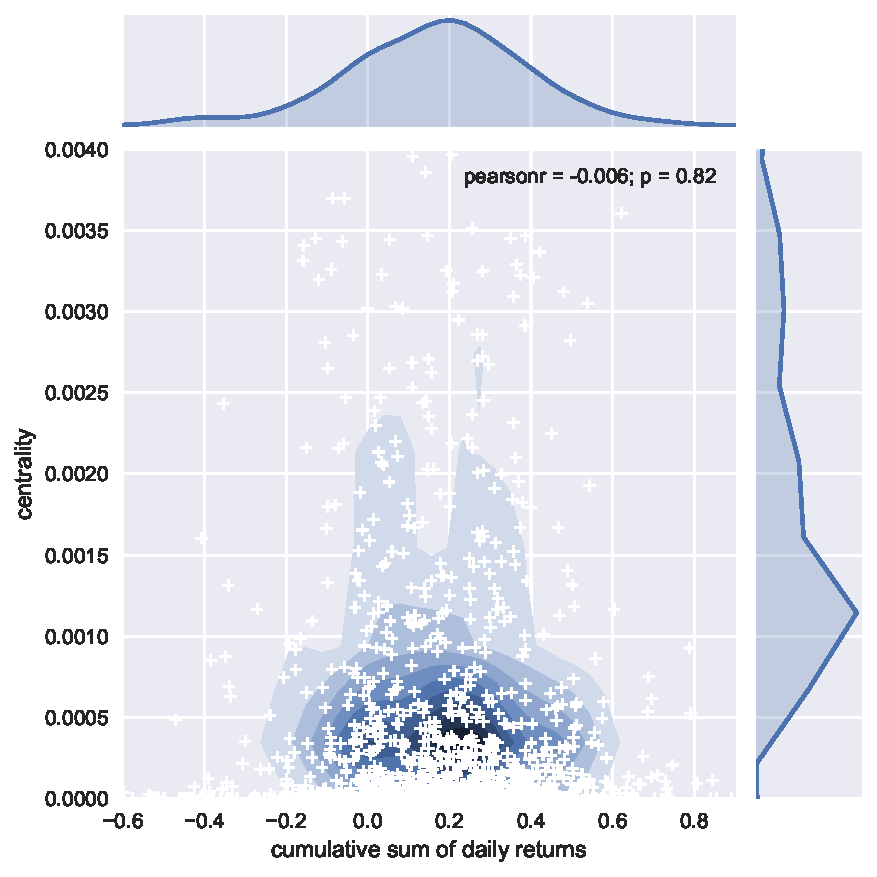
\includegraphics[width=0.46\textwidth]{sum_return_weighted_centrality}%
		\label{subfig:sum_return_weighted_centrality}%
	}%
	\hfill%
	\subfloat[Bivariate distribution beween betweenness centralities of nodes and standard deviations of stock daily return.]{%
		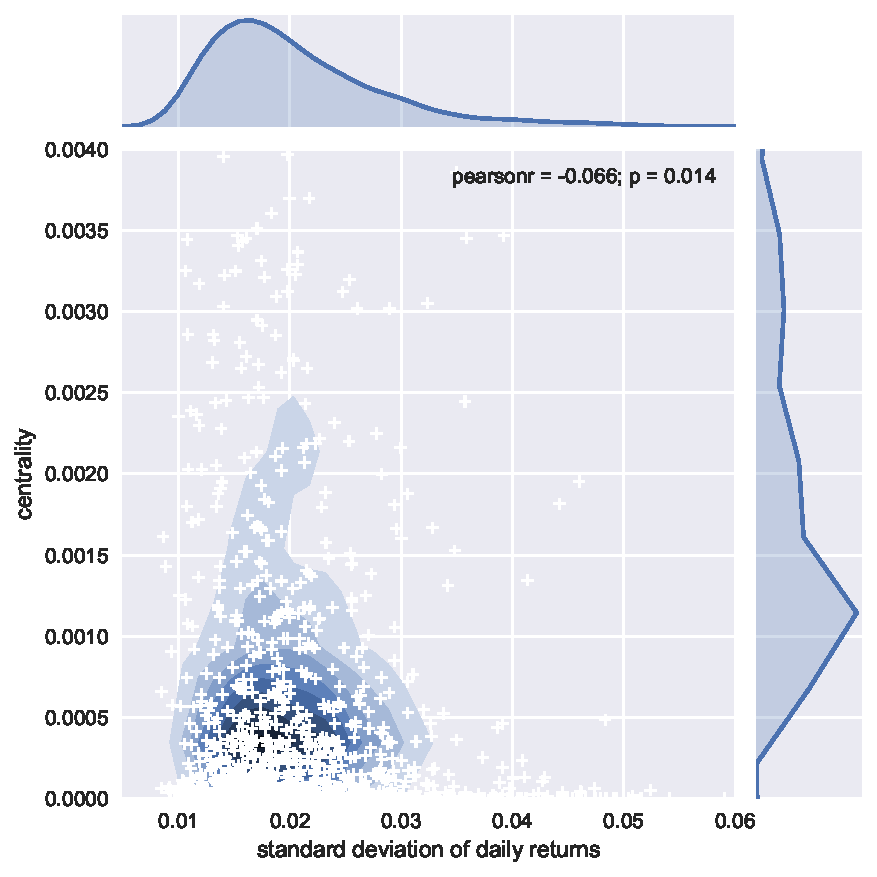
\includegraphics[width=0.465\textwidth]{std_return_weighted_centrality}%
		\label{subfig:std_return_weighted_centrality}%
	}%
	\caption{Bivariate distributions with betweenness centrality} \label{fig:bivariate}
\end{figure}

Figures~\ref{fig:bivariate} reveal the relationships between betweenness centralities and price returns of stocks. First, in figure~\ref{subfig:sum_return_weighted_centrality} as much more nodes have low betweenness centrality values (lower than $0.001$), and the cumulative sum of returns fall intensively in the range of $(-0.1, 0.6)$, while that of the nodes with high betweenness centrality values (higher than $0.001$) also fall evenly in the same range Therefore, there is no significant difference between the expected return for stocks with different betweenness centrality values.

Second, according to the figure~\ref{subfig:std_return_weighted_centrality}, in spite of several outliers, as the betweenness centrality of nodes becomes higher, there will be a higher possibility of nodes tend to have low standard deviation of stock daily return. This indicates the hubs in the network have considerably stable return during the specified researched year among the whole stock market. The average standard deviation for all values of betweenness centrality remain similar because of the more frequent occurrences of outliers with higher betweenness centralities from the figure.

As a result, although choosing stocks with high centralities possibly will not bring a higher expected return for a portfolio, they have the functionality of decreasing the overall risks and generating more stable returns, which is also a vital feature for stock investment.


%\label{sec:community}
%\section{Stability of network}

%Industry

